
\documentclass[a4paper]{article}
\usepackage{pslatex}
\usepackage[T1]{fontenc}
\usepackage[utf8x]{inputenc}
\setlength\parskip{\medskipamount}
\setlength\parindent{0pt}
\usepackage{graphicx}
\usepackage{amssymb}
\usepackage{lscape}
%\usepackage{hyperref}

\usepackage{multicol}

\makeatletter

\providecommand{\boldsymbol}[1]{\mbox{\boldmath $#1$}}
\newcommand{\ASL}			{ASL}
\newcommand{\OSC}[1]		{\texttt{#1}}
\newcommand{\lra}			{$\leftrightarrow$}
\newcommand{\seg}[1]		{Seg(#1)}

\setlength{\parskip}{1mm}

\makeatother

\begin{document}

\title{FaustPlayground \\ v.1.0}

\author{Grame, Centre National de Création Musicale\\
{\small <research@grame.fr>} \\
\vspace{2mm}
[ANR-12-CORD- 0009] and [ANR-13-BS02-0008]
}

\maketitle

\topskip0pt

\newpage
\tableofcontents

\newpage
\section{General Considerations}

\subsection{FaustPlayground}
FaustPlayground is a web platform aiming to create patchs of Faust applications and export the patch as a unique application through the FaustWeb compilation service. \\

The FaustPlayground is an extension of the Web Audio Playground by Chris Wilson : http://webaudioplayground.appspot.com/ \\

Two versions of the interface have been created :
\begin{itemize}
\item The pedagogical version aims to introduce the notion of programmation to the young public, through the creation of an audio application. This application can be downloaded on a smartphone, once created.

\item The "normal" version is for every Faust user wanting to try online some  Faust examples, create patchs and use the export interface to FaustWeb service.
\end{itemize}

\subsection{Code Structure}

The scene is the principal element of the FaustPlayground. It is an audio and graphical container. The scene is implemented following the C++ class model, describing a serie of functions that can be executed on it (c.f. SECTION ??).

For the needs of both playgrounds, various scene instances are created:
\begin{itemize} 
\item For the pedagogical version: Accueil, Pedagogie, Finish
\item For the normal version: Playground
\end{itemize}

Those files implement specific functions creating the graphical elements to be added to the specific scene.
For each scene, we have three main functions :
\begin{itemize}
\item init: create the graphical elements
\item onload: callback whenever the scene is loaded in the page
\item onunload: callback whenever the scene is unloaded from the page
\end{itemize}
 
 Main.js handles the different scenes of the application and the navigation between them. \\
 
 The second main element of the FaustPlayground is the notion of Module, representing a Faust application and it's interface.

\section{SceneClass.js}

\subsection{Class Description}
The SceneClass is an audio and graphical container for Modules. \\

In order to create a scene, you will have to call: {\it createScene(identifier, onload, onunload)}\\
The identifier will become the identifier of the container DIV. Onload/Onunload are callbacks for whenever the scene is loaded/unloaded from the page.

The fields of this class are:
\begin{itemize}
\item Input/Output: intermediate input/output Faust Modules to simplify mute/unmute scene
\item Modules: list of modules contained in the scene
\end{itemize}

The public methods are:
\begin{itemize}
\item Delete scene
\item Add Input/ Add Output: add audio input/output Faust Modules
\item Integrate scene: integrate scene to the page
\item Show/hide
\item Mute/unmute: connect/disconnect scene Input/Output to the WebAudio Context Input/Output
\item Add/Remove module
\item Get Modules
\item Clean Modules
\item Start/stop scene: execute onload/onunload callbacks
\item Get scene container
\item Get Input / get Output
\item Save/Recall scene: Through a Json Description, the scene can be saved and recalled (c.f SECTION ??)
\end{itemize}

\subsection{Scenes Instances}
\subsubsection{Pedagogical Version}
In the pedagogical, 3 scenes are created: Accueil, Pedagogie and Finish.
They correspond to the graphical menus in which we navigate in the pedagogical FaustPlayground.

\subsubsection{Normal Version}
In the normal version, a unique scene is created: Playground.

\section{Main.js}

 Main.js handles the different scenes of the application and the navigation between them.

\section{ModuleClass.js}

\section{Connect.js and Dragging.js}


\section{Pedagogie}
Specifically for the use of the Pedagogical Playground,



\section{Scenario - Example}

\section{Annexes}
\subsection{File interactions}
\begin{landscape}
\begin{figure}[!h]
\begin{center}
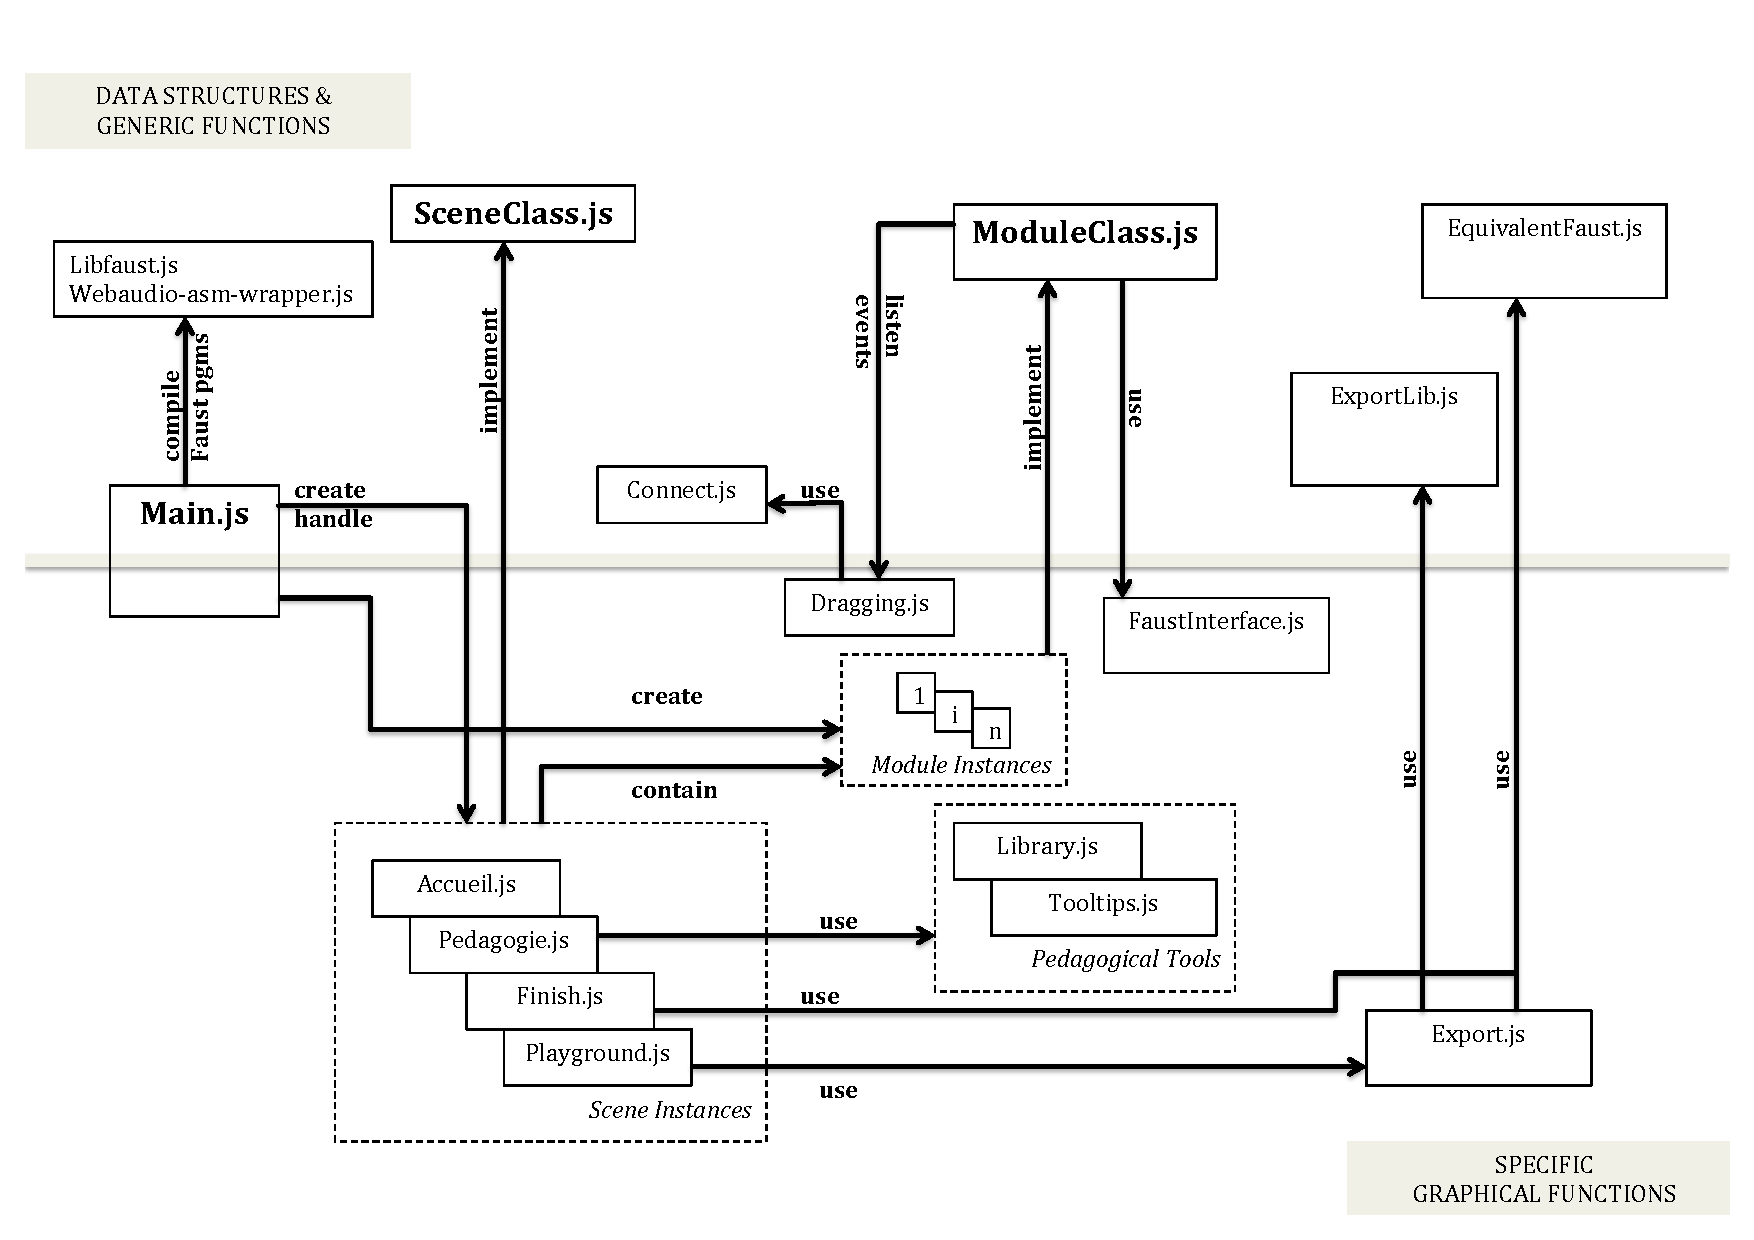
\includegraphics[width=\columnwidth]{images/ClassDiagram.pdf}
\label{fig:classes}
\end{center}
\end{figure}
\end{landscape}

\subsection{JSON Description for the scene}

\begin{figure}[!h]
\begin{center}
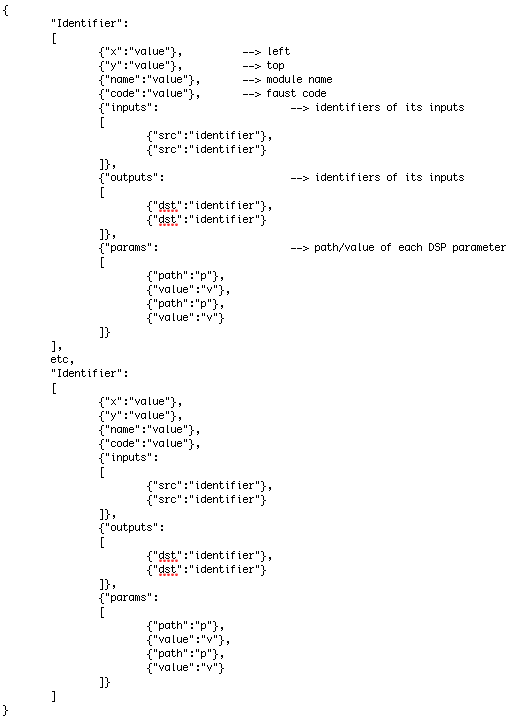
\includegraphics[width=\columnwidth]{images/JSON.png}
\label{fig:JSON}
\end{center}
\end{figure}


\end{document}




